\documentclass[12pt]{article}
\usepackage[utf8x]{inputenc}
\usepackage{amsmath}
\usepackage{graphicx}
\usepackage{hyperref}
\hypersetup{
	colorlinks=true,
	linkcolor=black,
	filecolor=black,      
	urlcolor=blue,
	citecolor=blue,
}

\begin{document}
	
	\begin{titlepage}
		
		\newcommand{\HRule}{\rule{\linewidth}{0.5mm}} % 
		\center 
		
		%----------------------------------------------------------------------------------------
		%	HEADING SECTIONS
		%----------------------------------------------------------------------------------------
		
		\textsc{\LARGE University of Milan}\\[0.5cm]
		\textsc{\Large Department of computer science}\\[0.5cm] 
		%----------------------------------------------------------------------------------------
		%	TITLE SECTION
		%----------------------------------------------------------------------------------------
		
		\HRule \\[0.4cm]
		{ \huge \bfseries Artificial Intelligence for Videogames project report}\\[0.4cm] % Title of your document
		\HRule \\[1.5cm]
		
		%----------------------------------------------------------------------------------------
		%	AUTHOR SECTION
		%----------------------------------------------------------------------------------------
		
		\Large \emph{Author:}\\
		Diego \textsc{Vallauri}\\[2cm]
		
		%----------------------------------------------------------------------------------------
		%	LOGO SECTION
		%----------------------------------------------------------------------------------------
		
		
\includegraphics[scale=0.2]{images/logo.png}\\[1cm] 
		
		%----------------------------------------------------------------------------------------
		
		\vfill 
		
	\end{titlepage}

	\tableofcontents
	
	\newpage
	
	\section{Introduction and purpose of the project}
	The project started with reference to the \textbf{Pong} game, where there are two players whose aim is to hit the ball without being overtaken by it. Starting from this, we decided the purpose of the project, which is to create an agent who can take the place of a player. In short, my goal was to create an agent who would hit the ball every time without missing it.
	To solve the problem, the first idea I proposed was a trigonometric solution. Since it wasn't that easy to put into practice, the Teacher suggested to use \textbf{Machine Learning} instead. This is the solution I adopted to the project and in particular I relied on \textbf{TensorFlow} which acts as an intermediary between Unity and Machine learning itself.\\
	At the end of the project, I created three agents. The first moves only left and right (as in the \textbf{Pong} game), the second agent and the third in each four directions. Since the third was probably not required for the project, I consider it as an experiment I did towards the end.
	
	\newpage
	
	\section{Creation of the environment}
	Since the aesthetic part was not part of the project, I only used some Cubes and Cylinders to create the environment, as can be seen in the image below of the agent and the disk.
	
	\begin{figure}[hbt!]
		\centering
		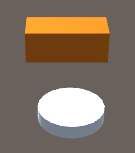
\includegraphics[width= 0.3
		\textwidth]{images/Disk&Agent}
	\end{figure} 

	\noindent
	I have created two types of fields. One for training and one with two agents. I will explain the use of these fields in the next section.

	\begin{figure}[hbt!]
		\centering
		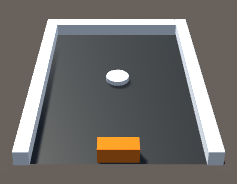
\includegraphics[width= 0.70
		\textwidth]{images/TrainingField2}
		\caption{This is the field for training with just one side open.}
		\label{lbl:traningField}
	\end{figure} 
	
	\newpage
	
	\begin{figure}[hbt!]
		\centering
		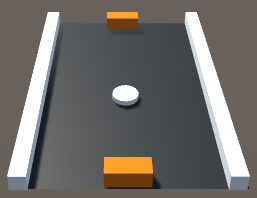
\includegraphics[width= 0.70
		\textwidth]{images/AgentVsAgentField2}
		\caption{This is the normal field with two open sides.}
	\end{figure} 
	
	\newpage
	
	\section{First agent}
	The folder that describes the agent and the environment of this first example is located in \textbf{"Asset/FistTest"}.
	
	\subsection{Environment set up.}
	Before starting to train the agent, I obviously need to set my field. For the training I will use the \textit{training field} (Figure \ref{lbl:traningField}). The first thought to decide is how to bounce the disk off the walls. Since every wall has a \textit{Collider} and the disk a \textit{RigidBody}, we can let the physics engine do it for us. Obviously I have to help it and have to make some considerations. For example, I don't want friction between the plane and the disk and between the disk and the wall.
	I also don't want the disk to stop moving after colliding with multiple walls.
	From this base, I created two different physical materials, each without friction but one with a bounciness equal to 1 and one equal to 0 (I don't want the disk to bounce on the plane). I assigned the first material to the side walls and the second to the floor.
	
	\begin{figure}[hbt!]
		\centering
		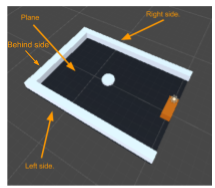
\includegraphics[width= 0.73
		\textwidth]{images/SidePlane.png}
		\caption{Representation of side walls and the plane.}
		\label{lbl:SidePlane}
	\end{figure} 
	
	\newpage
	
	\begin{figure}[hbt!]
		\centering
		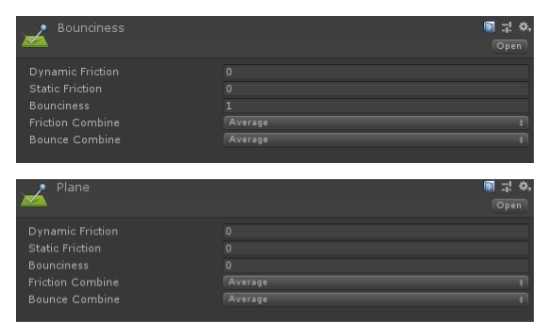
\includegraphics[width= 1
		\textwidth]{images/PM.png}
		\caption{Physic material of the walls and the plane.}
	\end{figure} 

	\noindent
	Now there is the "hardest" part: how do I make the disk bounce with the agent in a real way?
	First of all, I can't let the physics engine work because the disk will always behave the same way. I mean, if the ball goes straight through the middle to the agent, the ball will continue to change its Z coordinate but the X would remain the same (or at least, very similar. See figure \ref{lbl:mvmupdown}) and in a nutshell its movement will remain the same.
	My solution is to look for the new destination and then add a force in that direction. For this, I used the Vector3.reflect function, which takes two parameters: in-direction and normal. In short I will calculate a new position that reflects the direction of the ball on the normal of the impact.
	
	\newpage
	
	\begin{figure}[hbt!]
		\centering
		\includegraphics[width= 0.4
		\textwidth]{images/FieldmovementUpDown.png}
		\caption{The only possible movements if the disk start straight to the agent.}
		\label{lbl:mvmupdown}
	\end{figure} 

	\begin{figure}[hbt!]
		\centering
		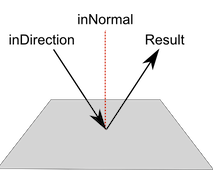
\includegraphics[width= 0.5
		\textwidth]{images/Reflect.png}
		\caption{In summary, this is what the \textbf{Vector3.reflect} function returns.}
		\label{lbl:reflect}
	\end{figure} 
	
	\noindent
	So after find the new destination, I will apply a force based on new vector normalized and the speed of the disk.
	The code for this part is on the next page. As you will see, there is also an "OnTriggerEnter", whose sole purpose is to set the \textbf{haveILose} variable to true if the disk passes the agent (there is a game object in the scene called "onTriggerGoal" with the check mark on the "isTrigger" in the collider). The  \textbf{haveILose} will be used on the agent for cheacking if the agent has lost and restart the episode, or not.
	
	\newpage
	
	\begin{figure}[hbt!]
		\centering
		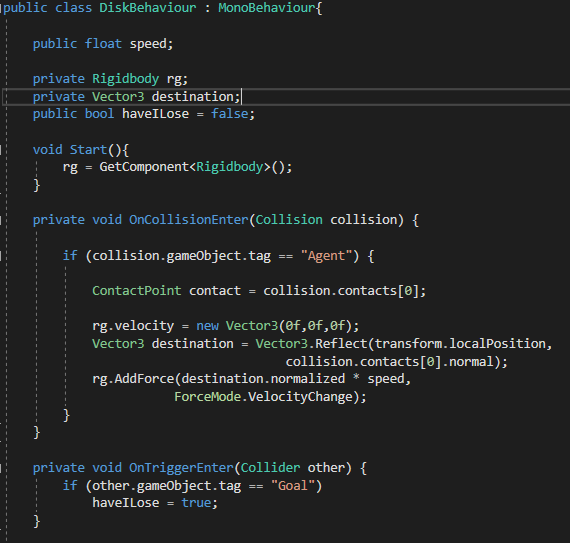
\includegraphics[width= 1
		\textwidth]{images/DiskBehaviour1.png}
		\caption{Disk behaviour class.}
		\label{lbl:reflect}
	\end{figure} 
	
	\noindent
	One last thing I forgot to mention, is that this behaviour is attached to the agent but also to the behind wall (figure \ref{lbl:SidePlane}), since in training it simulates a real agent.
	
	\subsection{Training set up}
	Now i am ready to create my agent. As suggested, I create an empty game object as parent of my parallelepiped. Since i wanted to use a \textbf{RigidBody} for the physics and wanted to keep the agent part and the movement divided,  I simply assigned everything about the agent to the parent and the \textbf{RigidBody} and collider to the child.  
	
	\begin{itemize}
		\item \textbf{Agent}: Has attached the \textbf{Behavior Parameters}, the \textbf{Decision Requester} and the \textbf{BAgent} (my script).
		\item \textbf{Player}: It is the son of \textbf{Agent} and has attached the \textbf{Box Collider}, the \textbf{RigidBody} and everything needed for rendering.
	\end{itemize}
	
	\noindent
	Let's now analyse the \textbf{BAgent} script. Since it extends the Agent class it has at least four methods: \textbf{Initialize}, \textbf{OnEpisodeBegin},\textbf{ CollectObservations},\textbf{ OnActionReceived}.\\
	
	\begin{itemize}
		\item \textbf{Initialize}: it has nothing special about it, just the initialization of the disk \textbf{RigidBody} and the agent child reference (that will actually move).	
		
		\begin{figure}[hbt!]
			\centering
			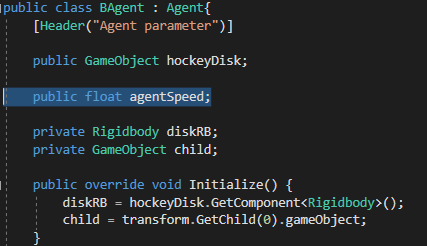
\includegraphics[width= 0.8
			\textwidth]{images/Initialize.png}
		\end{figure} 
	
		\item \textbf{OnEpisodeBegin}: I first take the value of \textbf{haveILose} and set it to false, since the true value is the trigger event for the end of the episode. So I create a different position for the agent, for the disk and calculate a new starting direction for the disk. At the end I add a force in the calculated direction.
		
		\newpage
		
		\begin{figure}[hbt!]
			\centering
			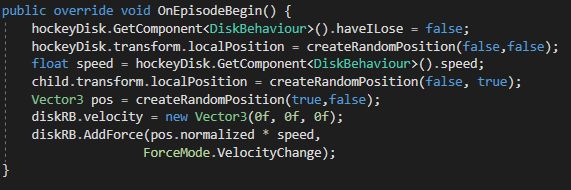
\includegraphics[width= 1
			\textwidth]{images/OnEpisodeBegin.png}
		\end{figure} 
	
		The \textbf{createRandomPosition} method, is only an auxiliary method to create the position of the elements based on the parameters. (It's not that interesting so I don't put any photos there, but it's obviously present in the folder).
		
		\item \textbf{CollectObservations}: this is quite important and contains seven observations. The first three are the component of the local position of the disk, The fourth is the \textit{x} local position of the agent and the last three are the component of the RigidBody velocity.\\
		In this part I made some mistake at the beginning, for example I gave the global and not the local position of the elements and this create problems during the training because every prefabs has it's own global position and so the learning didn't go very well. Another mistake (not really a mistake) was providing the agent \textit{y} and \textit{z} components as well (which are fixed) and this only slowed down the training.
		
		\begin{figure}[hbt!]
			\centering
			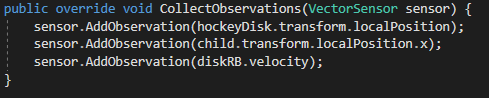
\includegraphics[width= 1
			\textwidth]{images/CollectObservation.png}
		\end{figure}
	
		\item \textbf{OnActionReceived}: the agent will receive only a float (clamped beetween -1 and 1) and will first reset the RigidBody velocity of the agent and then add a force in the direction received before. \\
		Moreover the agent will receive a positive reward of 0.05 if the disk has not overcome it or a negative reward of -5 in the opposite case.
		
		\newpage
		
		\begin{figure}[hbt!]
			\centering
			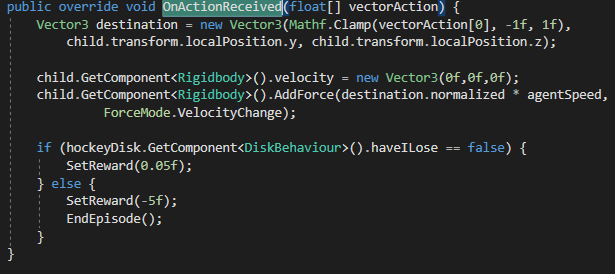
\includegraphics[width= 1
			\textwidth]{images/OnActionReceived.png}
		\end{figure}
		
	\end{itemize}	
	
	\subsection{The training}
	For the learning i will use the scene \textbf{Test}.
	
	\begin{figure}[hbt!]
		\centering
		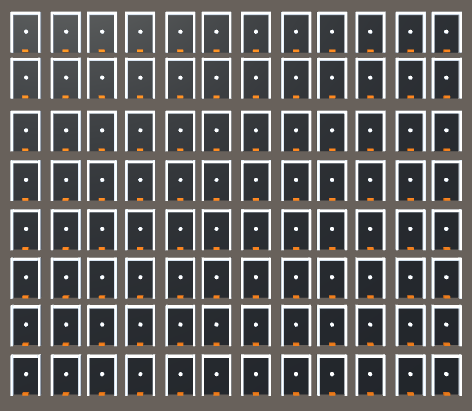
\includegraphics[width= 0.76
		\textwidth]{images/NormalTraining1.png}
		\caption{Scene \textbf{Test} with 96 field prefabs.}
	\end{figure}
	
	\newpage
	
	\noindent
	For the .yaml file, I followed the instruction on the \href{https://github.com/Unity-Technologies/ml-agents/blob/master/docs/Training-Configuration-File.md}{doc site}. 
	In particular in this first example the .yaml file is composed in that way:
	
	\begin{figure}[hbt!]
		\centering
		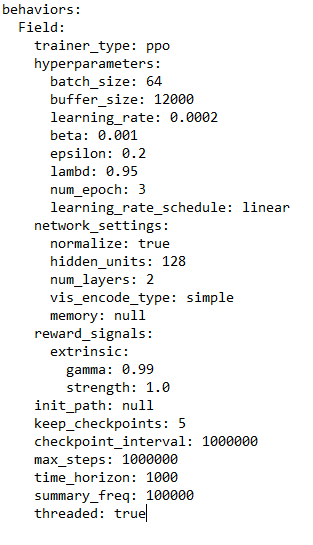
\includegraphics[width= 0.6
		\textwidth]{images/Behaviour.png}
		\caption{Behaviour.yaml}
	\end{figure}
	
	\noindent	
	As can be seen from above, the learning lasted 1000000 steps. \\
	Learning works very well and the agent is able to hit the ball every time (see the video "\textbf{FirstTestTraining}" in the folder). \\
	After the first training session, I panicked when I tried to play against another agent. In this case, the one in the opposite position of the training could not catch the ball. At first I thought it was my mistake, but after a few tries I think the problem was only in the reference system. If we take for example the output "-1" of the neural network for the normal agent it indicates to go to the left, while for the "inverse" agent it indicates to go right. I suppose that was the problem, but maybe it's something I don't catch.
	
	\begin{figure}[hbt!]
		\centering
		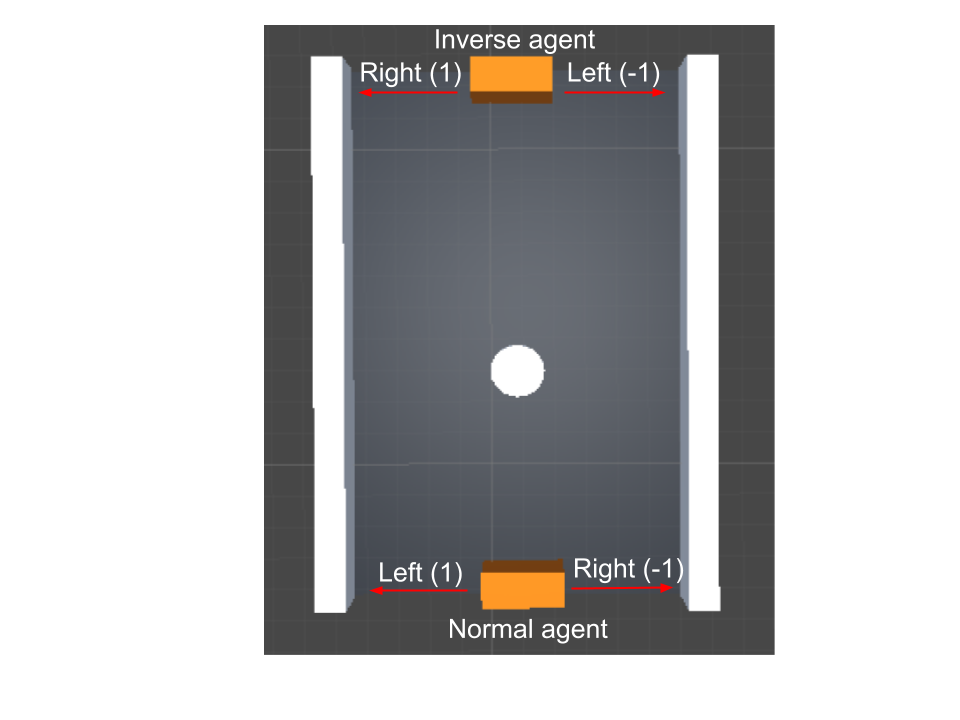
\includegraphics[width= 1
		\textwidth]{images/AvsA.png}
		\caption{Different reference system for the two agents.}
	\end{figure}
	
	\noindent
	 So, to create the second agent, I did the same training as before with the agent in the opposite position.
	 \newpage
	
	\begin{figure}[hbt!]
		\centering
		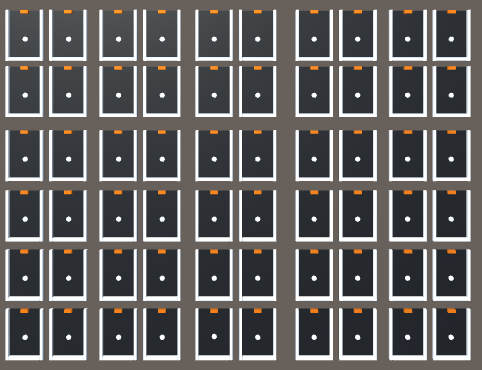
\includegraphics[width= 0.76
		\textwidth]{images/InverseTraining1.png}
		\caption{Scene \textbf{InverseTest} with 60 field prefabs.}
	\end{figure}
	
	\noindent
	Now after assign the two brains to the different agents, they could play together without any problems. (see "\textbf{AgentVSAgentTest1}" video).
	Since I wanted to create only one brain for the two agents, I decide to do a mixed training with half normal field and half inverse field. The results is pretty good and its behaviour it's very similar to the initial brain (see "\textbf{AgentVSAgentSameBrain}" video). Obviously the learning rate it's a little bit slower and it's not as accurate as the normal training, but it's ok.
	
	\newpage
	
	\begin{figure}[hbt!]
		\centering
		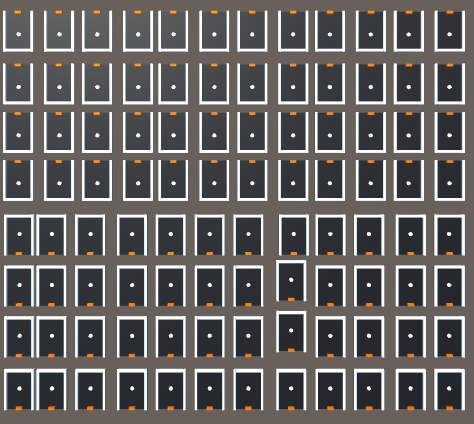
\includegraphics[width= 0.76
		\textwidth]{images/MixedField.png}
		\caption{Scene \textbf{MixedTest} with 48 normal field prefabs and 48 inverse field prefabs.}
	\end{figure}

	\subsubsection{Conclusion}
	In conclusion, the first experiment went very well and I created an agent that is able to hit the disk every time without any particular problems.
	
	\newpage
	
	\section{Second agent}
	
	The next stage is to create an agent that can move in every four directions. The folder that describes the agent and the environment of this second example is located in \textbf{"Asset/SecondTest"}.
	
	\subsection{Environment set up.}
	
	Referring to the "\textbf{Normal}" scene, there are some small changes. There is a new empty game object called "\textbf{Middle Field}" with only a box collider to use as a limit for the movement of the player in the center of the field. There is actually a duplicate of the component used to restrict player movement at the bottom of the pitch.
	
	 \begin{figure}[hbt!]
	 	\centering
	 	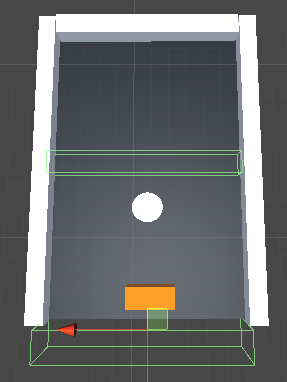
\includegraphics[width= 0.59
	 	\textwidth]{images/MiddleField.png}
	 	\caption{Gizmos of the box collider of the two new "\textbf{Middle Field}" game object.}
	 \end{figure}
	
	\noindent
	Also, there is a script attached to the game object whose sole purpose is to ignore the collision for the disk. If I didn't, the disk would stop shortly after the episode started.
	
	\begin{figure}[hbt!]
		\centering
		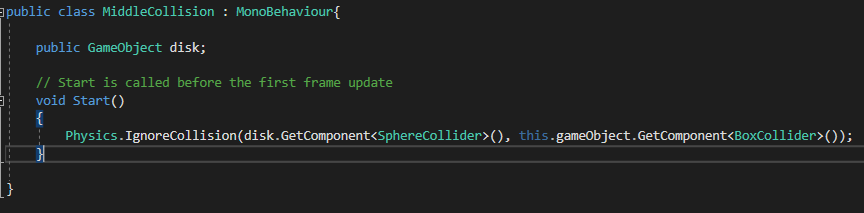
\includegraphics[width= 1
		\textwidth]{images/MiddleCollisionCode.png}
		\caption{MiddleField's script.}
	\end{figure}
	
	\noindent
	The second change is in "\textbf{DiskBehaviour2}". The script is very similar to the one in the first test folder, but when the disk collides with the agent, the behind wall is randomly placed in his half court. I think it can help the agent learn better since his opponent can have different \textit{z} coordinates and not stand still in the same position.
	
	\begin{figure}[hbt!]
		\centering
		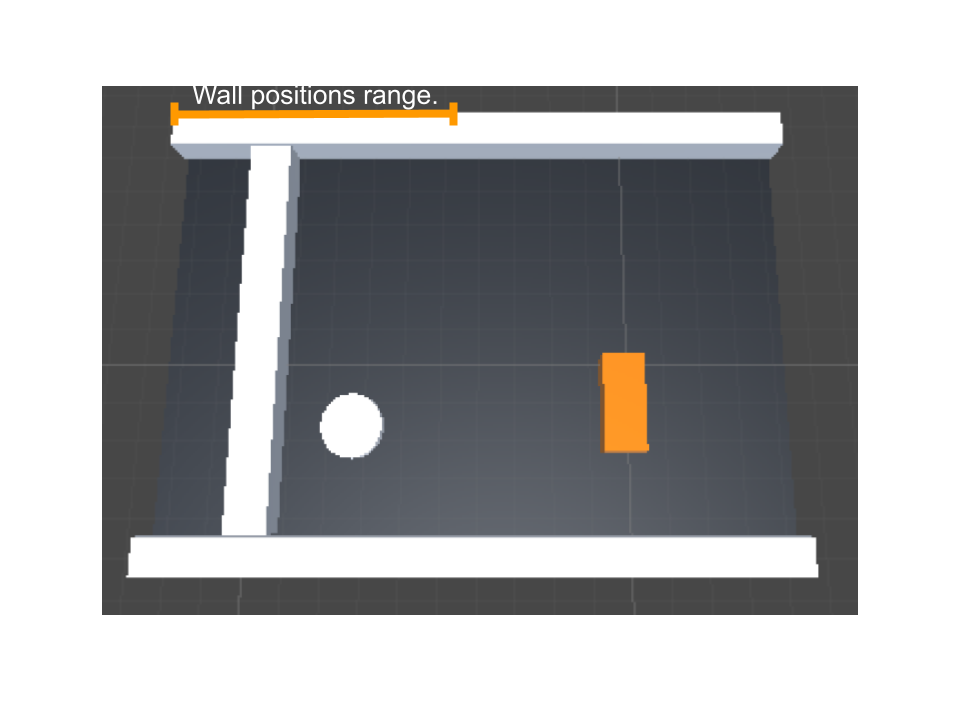
\includegraphics[width= 0.82
		\textwidth]{images/BehindWall.png}
		\caption{Representation of the different position of the wall.}
	\end{figure}
	
	\noindent
	The only thing that changes in the script is in the \textbf{OnCollisionEnter} method. It is just an if that checks the position of the wall and adds a random position (the if is needed to also work in the "inverse field" for the training of the second agent).
	
	\begin{figure}[hbt!]
		\centering
		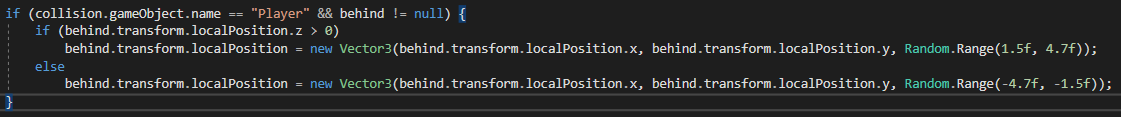
\includegraphics[width= 1.25
		\textwidth]{images/DiskBehaviour2.png}
		\caption{Code added in the \textbf{OnCollisionEnter} method.3}
	\end{figure}

	\subsection{Training set up}
	
	Also in the training set up there are some small changes in the different method of the agent (script: \textbf{BAgent2}).
	
	\begin{itemize}
		\item \textbf{Initialize}: same as before.
		
		\item \textbf{OnEpisodeBegin}: As new there is the "if" to change the position of the behind wall. The "if" is done only if we are using a field with a behind wall, in the other case the "\textbf{training}" variable is set to false.
		
		\begin{figure}[hbt!]
			\centering
			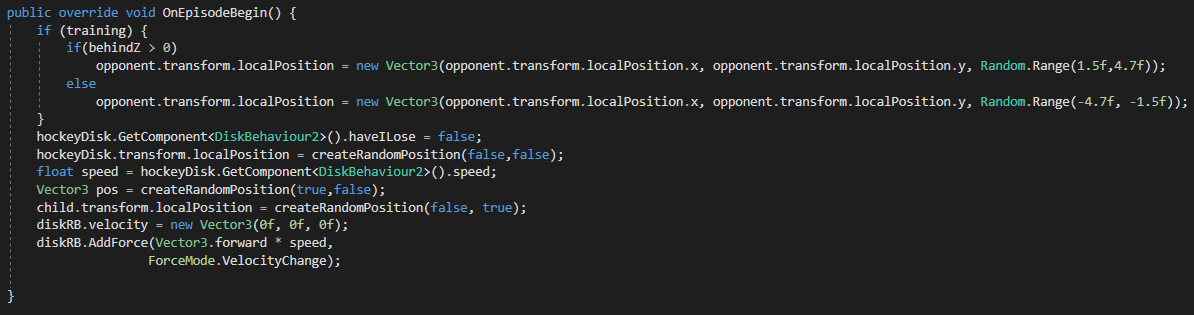
\includegraphics[width= 1.25
			\textwidth]{images/OnEpisodeBegin2.png}
		\end{figure}
		
		\item \textbf{CollectObservations}: in addition to the seven observations we sent in the first example, we also send the \textit{z} coordinate of the agent's local position. I tried to give the \textit{z} coordinate of the behind wall local position as an observation, but it was irrelevant to the neural network output, so I took it out.
		
		\newpage
		
		\begin{figure}[hbt!]
			\centering
			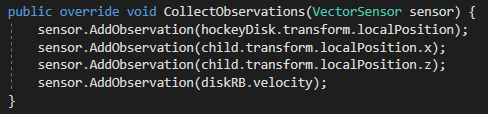
\includegraphics[width= 1
			\textwidth]{images/CollectObservation2.png}
		\end{figure}
		
		\item \textbf{OnActionReceived}: in addition to the float for the \textit{x} coordinate, the agent will receive a float (always clamped beetween -1 and 1) for the \textit{z} coordinate. 
		
		\begin{figure}[hbt!]
			\centering
			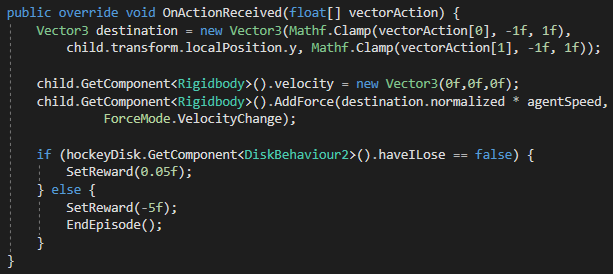
\includegraphics[width= 1
			\textwidth]{images/OnActionReceived2.png}
		\end{figure}
		
	\end{itemize}	
	
	\subsection{The training}
	The .yaml file used for the training is "\textbf{configuration.yaml}", which is the same file used before but the learning lasts 2000000 steps. That's probably a little too much, but since the training is a bit slower I preferred it that way.
	As before I created three different agent, the first is the one from the "\textbf{Test}" scene and it's the brain of the agent in the normal position. The second is the one in the inverse position and the third is the one with mixed training.
	Look at the different video of the agent in the folder.
	
	\subsection{Conclusion}
	Also in the second example went very well and the agent was able to hit the ball moving in all of the different four direction.
	
	\section{Last agent}
	I consider this last agent as an experiment and it's similar to the second example. The folder that describes the agent and the environment of this third example is located in \textbf{"Asset/ThirdTest"}.
	
	\subsection{Environment set up.}
	
	Different from before is that the pitch is a bit bigger and there is a goal to score at.
	
	\begin{figure}[hbt!]
		\centering
		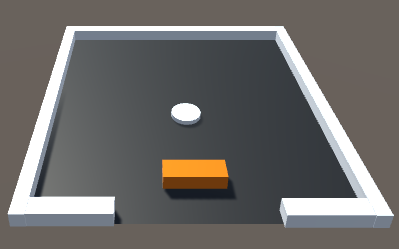
\includegraphics[width= 1
		\textwidth]{images/NewField.png}
	\end{figure}

	\noindent
	In the \textbf{DiskBehaviour3} script, it's the same as before, the only difference  is a check in the update method if the magnitude of the RigidBody velocity is less than 5. If so, it adds a force to the disk. This check is necessary in case the agent attempts to stop the disk in one of the lower side walls (and yes, he will try).
	
	\begin{figure}[hbt!]
		\centering
		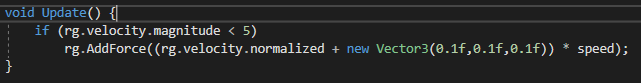
\includegraphics[width= 1
		\textwidth]{images/DiskBehaviour3.png}
	\end{figure}

	\subsection{Training set up}
	There are no change from the second example.
	
	\subsection{Training}
	I have called this third example as an experiment, because when i tried the learning i was thinking that everything would be ok. Instead the training has some problems. Since the agent have a positive reward if the disk don't reach the goal, during the training he will try to stop the agent in in one of the lower side walls in the two following way:
	
	\begin{figure}[hbt!]
		\centering
		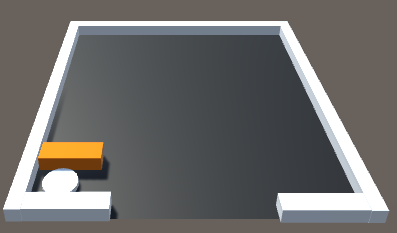
\includegraphics[width= 0.49
		\textwidth]{images/Obstacle1.png}
	\end{figure}

	\begin{figure}[hbt!]
		\centering
		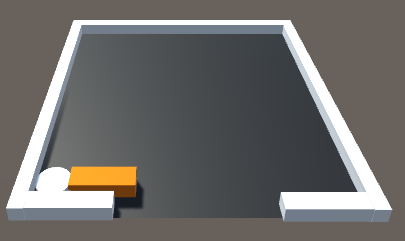
\includegraphics[width= 0.49
		\textwidth]{images/Obstacle2.png}
	\end{figure}
	
	\noindent
	There is also a second problem. In some training sessions the agent stays close to the centre of the pitch in a corner. This is because the disk has less change to go into the goal, which is smaller than before, so agents get a positive learning reward even if it doesn't try to hit the ball.
	
\end{document}	